\documentclass[working]{inputs/tuftebook}
\usepackage[utf8]{inputenc}
\usepackage[T1]{fontenc}
\usepackage{textcomp}

\usepackage{url}

\usepackage[
    sorting=nyt,
    style=alphabetic
]{biblatex}
\addbibresource{bibliography.bib}

\usepackage{hyperref}
\hypersetup{
    colorlinks,
    linkcolor={black},
    citecolor={black},
    urlcolor={blue!80!black}
}
\usepackage[noabbrev]{cleveref}

% Adds Bibliography, ... to Table of Contents
\usepackage[nottoc]{tocbibind}

\usepackage{graphicx}
\usepackage{float}
\usepackage[usenames,dvipsnames,svgnames]{xcolor}

% \usepackage{cmbright}

\usepackage{amsmath, amsfonts, mathtools, amsthm, amssymb}
\usepackage{mathrsfs}
\usepackage{cancel}

\newcommand\N{\ensuremath{\mathbb{N}}}
\newcommand\R{\ensuremath{\mathbb{R}}}
\newcommand\Z{\ensuremath{\mathbb{Z}}}
\renewcommand\O{\ensuremath{\emptyset}}
\newcommand\Q{\ensuremath{\mathbb{Q}}}
\newcommand\C{\ensuremath{\mathbb{C}}}
\let\implies\Rightarrow
\let\impliedby\Leftarrow
\let\iff\Leftrightarrow
\let\epsilon\varepsilon

\usepackage{tikz}
\usepackage{tikz-cd}

% theorems
\usepackage{thmtools}
\usepackage{thm-restate}
\usepackage[framemethod=TikZ]{mdframed}
\mdfsetup{skipabove=1em,skipbelow=0em, innertopmargin=12pt, innerbottommargin=8pt}

\theoremstyle{definition}

\makeatletter

\declaretheoremstyle[headfont=\bfseries\sffamily, bodyfont=\normalfont, mdframed={ nobreak } ]{thmgreenbox}
\declaretheoremstyle[headfont=\bfseries\sffamily, bodyfont=\normalfont, mdframed={ nobreak } ]{thmredbox}
\declaretheoremstyle[headfont=\bfseries\sffamily, bodyfont=\normalfont]{thmbluebox}
\declaretheoremstyle[headfont=\bfseries\sffamily, bodyfont=\normalfont]{thmblueline}
\declaretheoremstyle[headfont=\bfseries\sffamily, bodyfont=\normalfont, numbered=no, mdframed={ rightline=false, topline=false, bottomline=false, }, qed=\qedsymbol ]{thmproofbox}
\declaretheoremstyle[headfont=\bfseries\sffamily, bodyfont=\normalfont, numbered=no, mdframed={ nobreak, rightline=false, topline=false, bottomline=false } ]{thmexplanationbox}

\declaretheoremstyle[headfont=\bfseries\sffamily, bodyfont=\normalfont, numbered=no, mdframed={ nobreak, rightline=false, topline=false, bottomline=false } ]{thmexplanationbox}


\declaretheorem[numberwithin=chapter, style=thmgreenbox, name=Definition]{definition}
\declaretheorem[sibling=definition, style=thmredbox, name=Corollary]{corollary}
\declaretheorem[sibling=definition, style=thmredbox, name=Proposition]{prop}
\declaretheorem[sibling=definition, style=thmredbox, name=Theorem]{theorem}
\declaretheorem[sibling=definition, style=thmredbox, name=Lemma]{lemma}
\declaretheorem[sibling=definition, style=thmbluebox,  name=Example]{eg}
\declaretheorem[sibling=definition, style=thmbluebox,  name=Nonexample]{noneg}
\declaretheorem[sibling=definition, style=thmblueline, name=Remark]{remark}




\declaretheorem[numbered=no, style=thmexplanationbox, name=Proof]{explanation}
\declaretheorem[numbered=no, style=thmproofbox, name=Proof]{replacementproof}
\declaretheorem[style=thmbluebox,  numbered=no, name=Exercise]{ex}
\declaretheorem[style=thmblueline, numbered=no, name=Note]{note}

% \renewenvironment{proof}[1][\proofname]{\begin{replacementproof}}{\end{replacementproof}}

% \AtEndEnvironment{eg}{\null\hfill$\diamond$}%

\newtheorem*{uovt}{UOVT}
\newtheorem*{notation}{Notation}
\newtheorem*{previouslyseen}{As previously seen}
\newtheorem*{problem}{Problem}
\newtheorem*{observe}{Observe}
\newtheorem*{property}{Property}
\newtheorem*{intuition}{Intuition}


\declaretheoremstyle[
    headfont=\bfseries\sffamily\color{RawSienna!70!black}, bodyfont=\normalfont,
    mdframed={
        linewidth=2pt,
        rightline=false, topline=false, bottomline=false,
        linecolor=RawSienna, backgroundcolor=RawSienna!5,
    }
]{todo}
\declaretheorem[numbered=no, style=todo, name=TODO]{TODO}


\usepackage{etoolbox}
\AtEndEnvironment{vb}{\null\hfill$\diamond$}%
\AtEndEnvironment{intermezzo}{\null\hfill$\diamond$}%

% http://tex.stackexchange.com/questions/22119/how-can-i-change-the-spacing-before-theorems-with-amsthm
% \def\thm@space@setup{%
%   \thm@preskip=\parskip \thm@postskip=0pt
% }

\usepackage{xifthen}

\makeatother

% figure support (https://castel.dev/post/lecture-notes-2)
\usepackage{import}
\usepackage{xifthen}
\pdfminorversion=7
\usepackage{pdfpages}
\usepackage{transparent}


\makeatletter
\newif\ifworking
\@ifclasswith{tuftebook}{working}{\workingtrue}{\workingfalse}
\makeatother

\newcommand{\incfig}[2][1]{%
    % \ifworking{\makebox[0pt][c]{\color{gray}{\scriptsize\textsf{#2}}}}\fi%
    \def\svgwidth{#1\textwidth}
    \import{./figures/}{#2.pdf_tex}
}

\newcommand{\fullwidthincfig}[2][0.90]{%
    % \ifworking{\makebox[0pt][l]{\color{gray}{\scriptsize\textsf{#2}}}}\fi%
    \def\svgwidth{#1\paperwidth}
    \import{./figures/}{#2.pdf_tex}
}



\newcommand{\minifig}[2]{%
    \def\svgwidth{#1}%
    \begingroup%
    \setbox0=\hbox{\import{./figures/}{#2.pdf_tex}}%
    \parbox{\wd0}{\box0}\endgroup%
    \hspace*{0.2cm}
}

% %http://tex.stackexchange.com/questions/76273/multiple-pdfs-with-page-group-included-in-a-single-page-warning
\pdfsuppresswarningpagegroup=1

\newcommand\todo[1]{\ifworking {{\color{red}{#1}}} \else {}\fi}
\newcommand\charlotte[1]{\ifworking {{\color{blue}{#1}}} \else {}\fi}

\author{Gilles Castel}



\usepackage{multirow}
\def\block(#1,#2)#3{\multicolumn{#2}{c}{\multirow{#1}{*}{$ #3 $}}}

% \overfullrule=1mm

\newenvironment{myproof}[1][\proofname]{%
  \proof[\rm \bf #1]%
}{\endproof}

\usepackage{pdfpages}
\usepackage{efbox}


\usepackage{lipsum}
\usepackage{parskip}
\usepackage{titletoc}

\usepackage{cmbright}
\usepackage{bm}

\makeatletter
\newcommand{\globalcolor}[1]{%
  \color{#1}\global\let\default@color\current@color
}
\makeatother

\AtBeginDocument{\globalcolor{white}}

\definecolor{nord}{HTML}{313847}

\pagecolor{nord}

\addbibresource{bibliography.bib}


\begin{document}

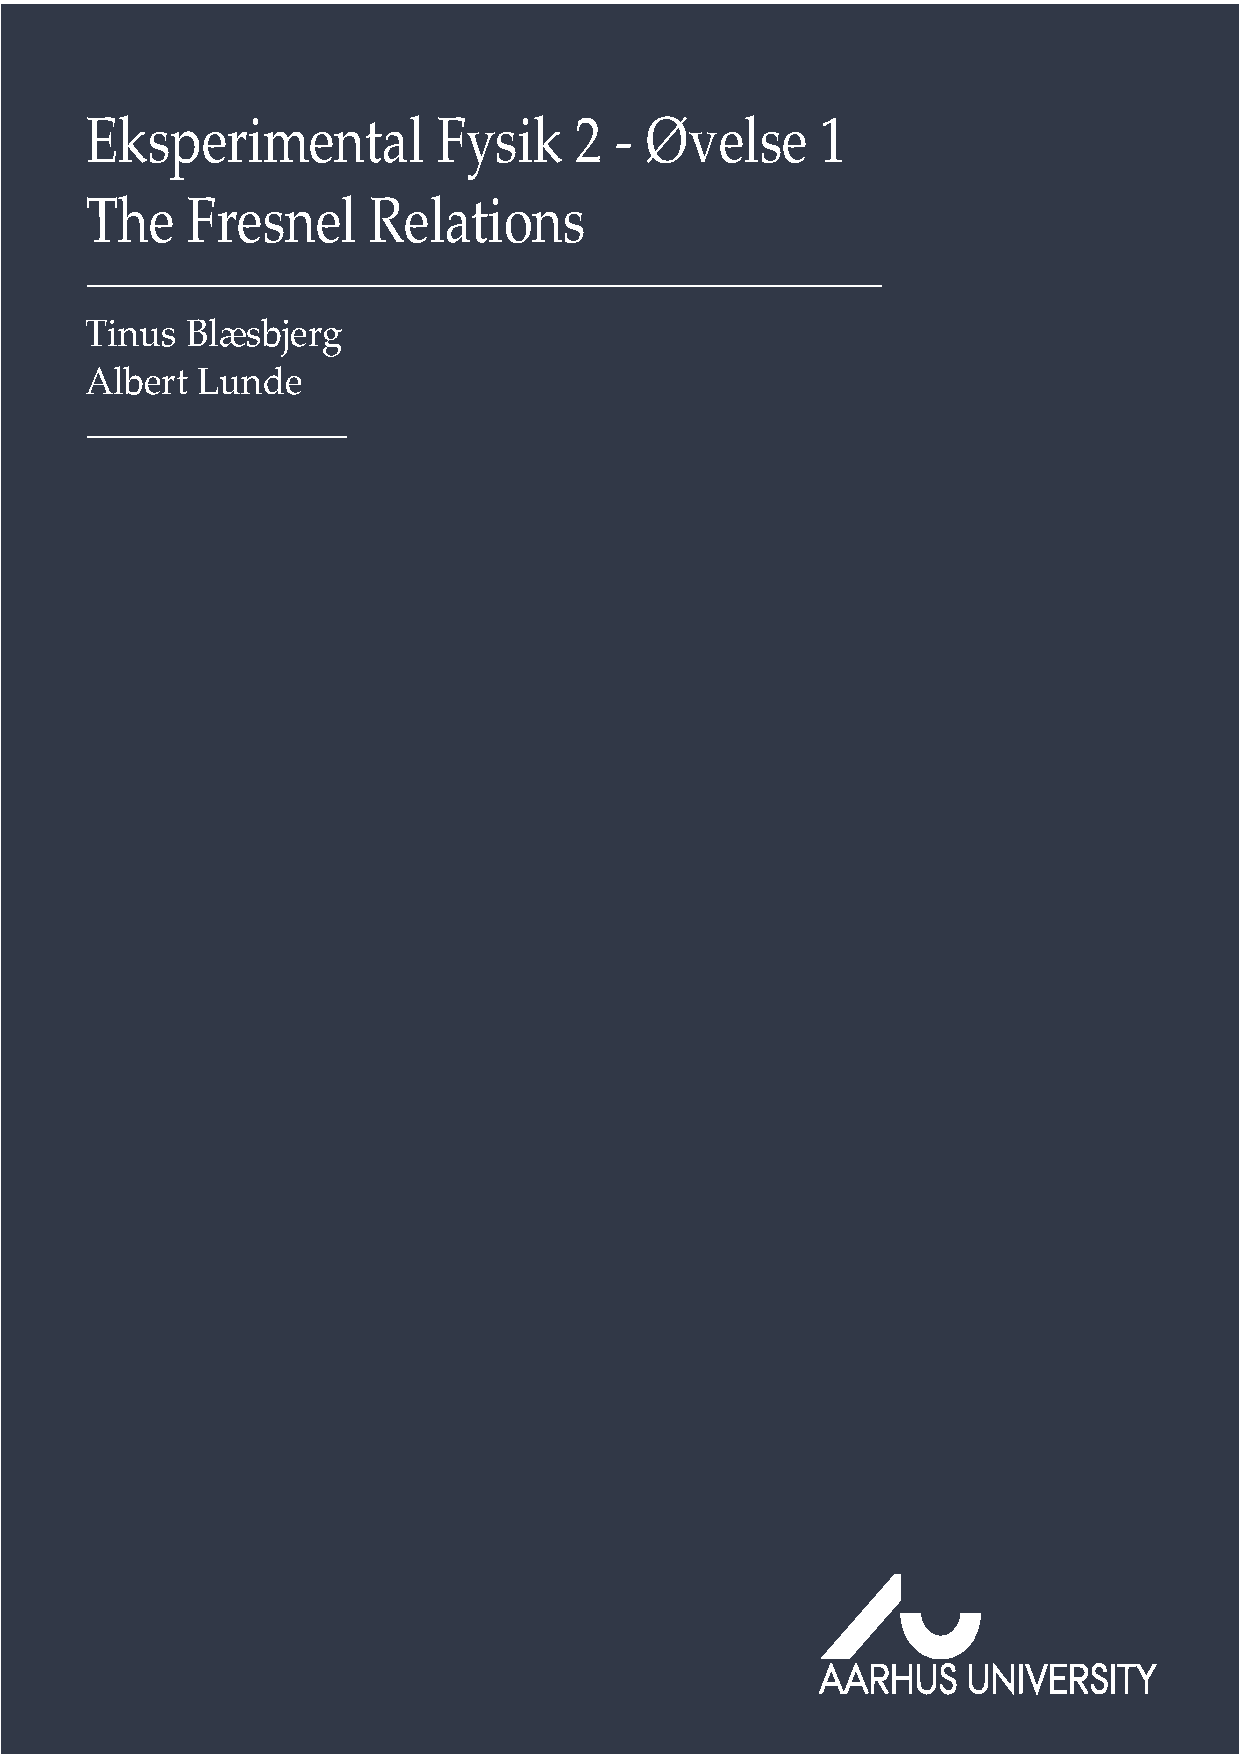
\includepdf[pages=-, fitpaper=true]{inputs/frontmatter.pdf}
\section*{Teori}
\subsubsection{Snell's Law}
When light passes through a dielectrica, the angle of reflection is equal to the angle of incidence, whereas the angle refraction is given by Snell's law;
\begin{marginfigure}
    \incfig{snell}
    \caption{Depiction of Snell's Law. As the light crosses the barrier between the two dielectrica, its angle changes. This angle is called the \textit{angle of refraction}.}
    \label{fig:snell}
\end{marginfigure}
\[
	\boxed{n_a \sin \theta_a = n_b \sin \theta_b}
\]
Where $n_a$ and $n_b$ are known as the indexes of refraction, which are properties of different materials. A materials index of refraction $n$ is related to the speed at which light moves through the material.
\[
n = \frac{c}{v}
\]
\subsubsection{Polarized light}
An electromagnetic wave consists of an oscillating electric field and an oscillating magnetic field. Since these fields are perpendicular and the propagation direction is perpendicular to both fields it is a transverse wave. Every electromagnetic wave has a certain orientation in space which can be determined by using the right hand rule. This can also be used to find the polarization of the wave, where the direction of the electric field determines the polarization. E.g if the orientation of the electric field is in the y-direction the wave is called linearly polarized in the y-direction.
\\
The visible light emitted from natural light source such as a light bulb or a laser is unpolarized. This means that the light consists of waves that are polarized in every possible direction. The light can be polarized in a specific direction by using a device called a polarizer. This device acts as a filter allowing only waves polarized in a specific angle through. Relevant for this experiment is when putting a polarizer rotated to 45 degrees in front of the laser, the electric and magnetic field of the light passing through can be split into two equally large components.

\begin{marginfigure}
    \incfig{polarized}
    \caption{The top figure depicts S-polarized light, while the bottom figure depicts P-polarized light.}
    \label{fig:polarized}
\end{marginfigure}
\begin{marginfigure}
    \incfig{fresnel1}
    \caption{The proportion of light that is transmitted and reflected is described by Fresnel's relations. For both $S$- and $P$-polarized light, a greater proportion is transmitted for most angles. Notice, that when the dielectrica has a circular, the light can pass through without changing direction} 
    \label{fig:fresnel1}
\end{marginfigure}
\subsubsection{Fresnel's Relations}
The angles of reflection and refraction are only part of the story. We are also interested in knowing how much of the incident light is reflected and transmitted. These intensities are given by the Fresnel relations, of which there are four. These relations describe the intensities of reflected and transmitted light for parallel and perpendicular polarized light. They have the following form;
\begin{align*}
	R_p &= \frac{\tan^2 \left( \theta_1 - \theta_2  \right) }{\tan^2 \left( \theta_1 + \theta_2  \right) }\\
	T_p &= \frac{sin(2\theta_1) sin(2\theta_2)}{sin^2(\theta_1+\theta_2)\cdot cos^2(\theta_1-\theta_2)}\\
	R_s &= \frac{\sin^2\left( \theta_1 - \theta_2 \right) }{\sin^2\left( \theta_1 + \theta_2 \right) } \\
	T_s &= \frac{sin(2\theta_1)sin(2\theta_2)}{sin^2(\theta_1 + \theta_2)}
.\end{align*}

If the energy is conserved then the sum of the intensity of all the different kinds of light should be equal to the intensity of the laser.
\subsubsection{Brewster's angle}
At a specific angle determined by the index of refraction of the two materials, the reflected light is polarized in the perpendicular direction of the plane of incidence. The relation is given in Brewster's law for the polarizing angle:
\begin{align*}
    tan(\theta_p) = \frac{n_b}{n_a}
\end{align*}
\begin{marginfigure}
	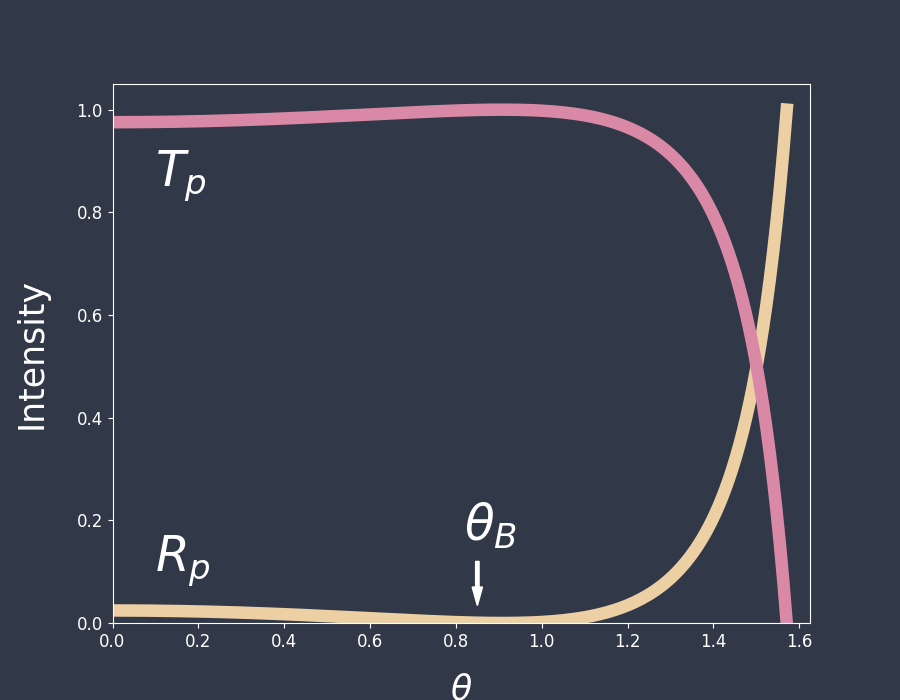
\includegraphics[width = 1.1\textwidth]{figures/fresnel2}
	\caption{This plot displays the intensities of the transmitted and reflected light. The transmitted light dominates for most angles. At tne brewster angle, all light is reflected. In this case, the index of refraction is 1.5 (glass).}
\end{marginfigure}
\subsubsection{The critical angle}
Another angle of interest is the critical angle, which can be derived from Snell's law of refraction by setting the refraction angle to 90 degrees:
\begin{align*}
    sin(\theta_{crit})=\frac{n_b}{n_a}
\end{align*}

At this angle no light is transmitted through the material. Instead the refracted light would move parallel with the demarcation line of the two materials. If the angle gets larger then total internal reflection occurs.

\begin{align*}
    T_p+T_s+R_p+R_s=I_{Laser}
\end{align*}
\begin{marginfigure}
    \incfig{fresnel3}
    \caption{At the \textit{critical angle} no light is transmitted. All of the light is reflected along the line separating the two materials. }
    \label{fig:fresnel3}
\end{marginfigure}
\section*{Experimental setup}
\begin{marginfigure}
    \incfig{setup}
    \caption{The setup used in the experiment.}
\end{marginfigure}
An illustration of the setup is shown in Figure 6.
\\
\subsection*{Material List}
\begin{itemize}
    \item Red Laser
    \item 2x Polarizer
    \item Dielectric
    \item Picoscope
    \item Turntable 
    \item Lens
    \item Light intensity detector with slit
\end{itemize}
The light from the laser moves through a polarizer set at an angle of 45\textdegree. This implies that the intensity of s- and p-polarized is equal. From the light impacts the dielectric where it is reflected and refracted. The light detector is moved to catch either the reflected or refracted. In front of the detector is a lens, which focuses the light, and anothera polarizer, which selects either s- or p-polarized light. The slit in front of the detector, changes the detectors sensitivity. In practice we move the turntable, keeping the dielectric fixed, until the intensity measured by the detector reaches a maximum. We then record the intensity, angle of incidence and angle of transmission/refraction.

\subsection*{Course of action}
In the experiment we want to examine different phenomena. These are:
\begin{itemize}
    \item Index of refraction.
    \item The relationship between the polarized light and the angle.
    \item The intensity of the total refracted light.
    \item The intensity of the total transmitted light.
    \item Conservation of the total intensity.
    
\end{itemize}
In order to test Fresnel's Relations we must know the index of refraction for the dielectric. Snell's law states that the index of refraction can be found from relation between the incidence and transmission angles. We therefore note transmission angle, for different angles of incidence. 
\\

When testing the conservation of the total intensity we can turn the dielectric and then measure the s- and p-polarized intensity for the transmitted and the reflected light. If the conservation is true, their sum should be constant. By noting the angles of incidence and transmission, we also use these measurements to test the Fresnel equation for e.g. the intensity of the p-polarized transmitted light. 
\subsection*{Error propagation}
Measurements that contains errors that should be considered include:
\begin{itemize}
    \item The angle 
    \item The background noise
    \item The width of the slit
\end{itemize}
 The most influential error in this experiment, is the one associated with the measurement of the angle. The protractor has a scale of 1 degreee, so the error must be $\pm 0.5$ \textdegree. Which when you propagate it. There is no reason to include the error of the sensor because when it was held steady it yielded an error of 0. The circular slit was used for all experiments and by using trigonometry we could determine that the error in the light actually hitting the center of the detector was negligible compared to the error in the protractor. The background noise was measured to be around 0.1 V for all angles and therefore also considered to be negligible compared to the intensity of the laser. When propagating the angle trough the function we used the functional method for the complex expressions and the analytic method for the less complex equations.
 \\
 
 Functional method:\sidenote{Measurements and Uncertainties, Ifan G. Hughes}
 \begin{align*}
     \alpha^A_Z & =f(\Bar{A}+\alpha_A,\Bar{B})-f(\Bar{A},\Bar{B}) ...\\
     &  (\alpha_Z)^2 = (\alpha^A_Z)^2 + (\alpha^B_Z)^2 ...
 \end{align*}
 
 Analytic method:
 \begin{align*}
     (\alpha_Z)^2=(\frac{\partial Z}{\partial A})^2(\alpha_A)^2 ...
 \end{align*}
\section*{Results}
What follows is a presentation of our data and results.
\subsubsection{Snell's Law}
Figure presents our data for Snell's law, we have plotted the sine of the incident angle againts the sine of the transmitted angle. Snells's law then predicts that the data is linear, with a steepness corresponding to,
\[
	\alpha = \frac{n_2}{n_1}
.\] 
\begin{figure}[h]
	\sidecaption{Graph depicting angles of incidence and refraction. The colored in area represents the uncertainty of the fit. The fit and uncertainty was decided using scipy's curve-fit function.}
	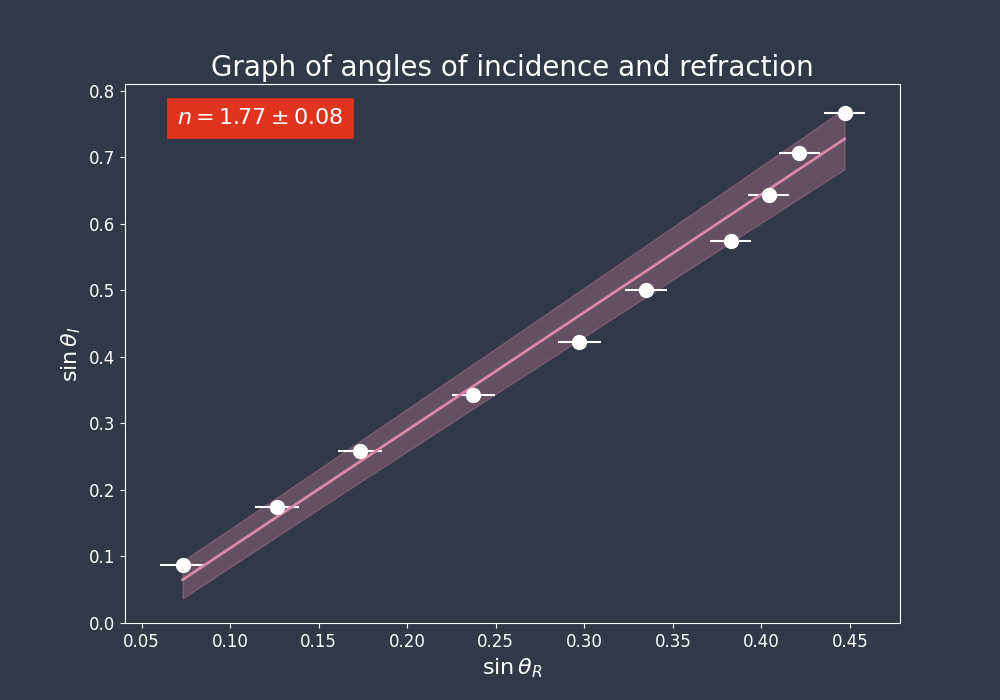
\includegraphics[width=\textwidth]{../snells-law}
	\label{fig:}
\end{figure}
As the plot shows, our data matches this quite well. We measure the value $n$ to be $1.77 \pm 0.08$, which is in the vicinity of what we would expect. We will be using this value and uncertainty in the remainder of the experiment, as Fresnel's relations rely upon it.
\subsubsection{Intensities}
Our data measuring the intensities also seems to follow the predicted curves reasonably well. We used the fact that,
\[
\theta_T = \arcsin \left( \frac{n_1}{n_2} \right) \theta_I
.\] 
To plot the theoretical curves for the Fresnel relations. Since we have measured the index of refraction with some uncertainty, this leads to an uncertainty in the predicted, which we have calculated using error propagation. We have also translated our uncertainty in angle to uncertainty in intensity using this same method. 
\begin{figure}[h]
	\centering
	\sidecaption{This graph shows the measured intensities of transmitted and reflected  p-polarized light at different angles $\theta_I$. Alongside this data is shown the curve predicted by Fresnels relations, the areas colored in represent the uncertainty in this theoretical curve. The uncertainty stems from our measurement of the refraction index. The data seems to follow the general shape of the curve.}
	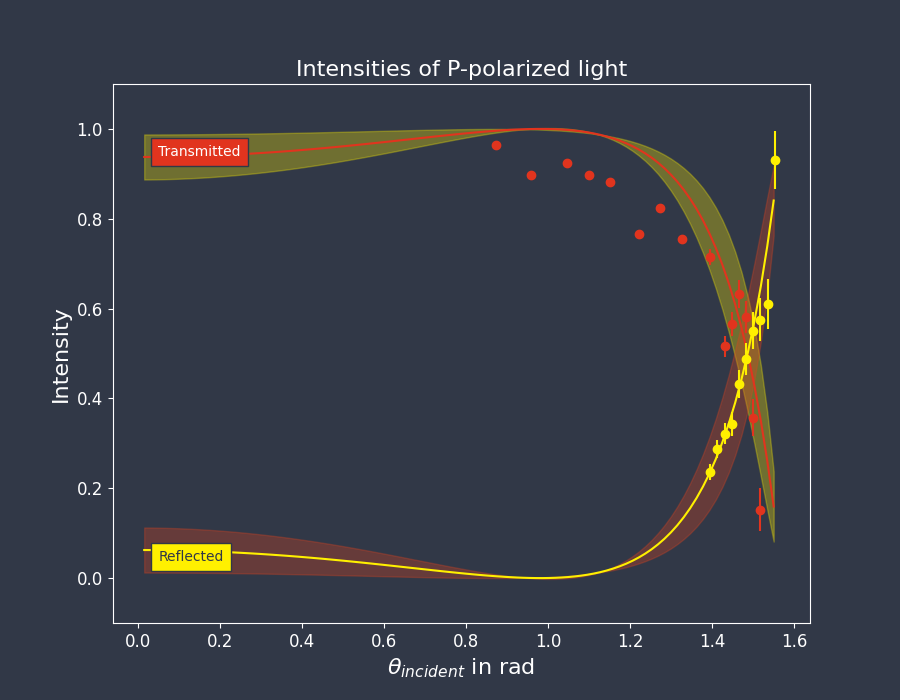
\includegraphics[width=\textwidth]{../RpTp}
\end{figure}
\begin{figure}[h]
	\centering
	\sidecaption{Plot of the S-polarized intensities. Once again, the data seems to follow curve reasonably. Interestingly the Fresnel relations for s-polarized light are more sensitive to the error in $n$.}
	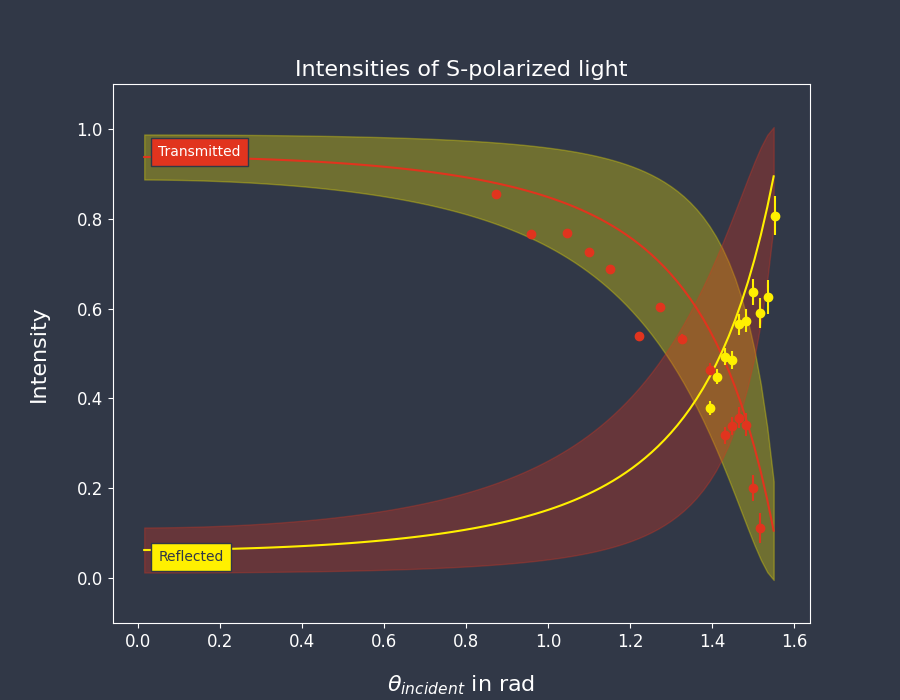
\includegraphics[width=\textwidth]{../RsTs}
\end{figure}
Note, that the lack of points at low angles of incidence is intentional. We chose to measure more points, where the curve should be steep and sensitive to change. 
\subsubsection{Conservation of intensity}
Lastly, we tested our hypothesis that,
\[
T_p + R_p = \text{constant} \quad \text{and} \quad T_s + R_s = \text{constant}
.\]
\begin{figure}[H]
	\centering
	\sidecaption{Fit of the sums of the intensities for p-polarized light. The data was fit to a linear function, and the fit did not yield a slope in the vicinity of 0.}
	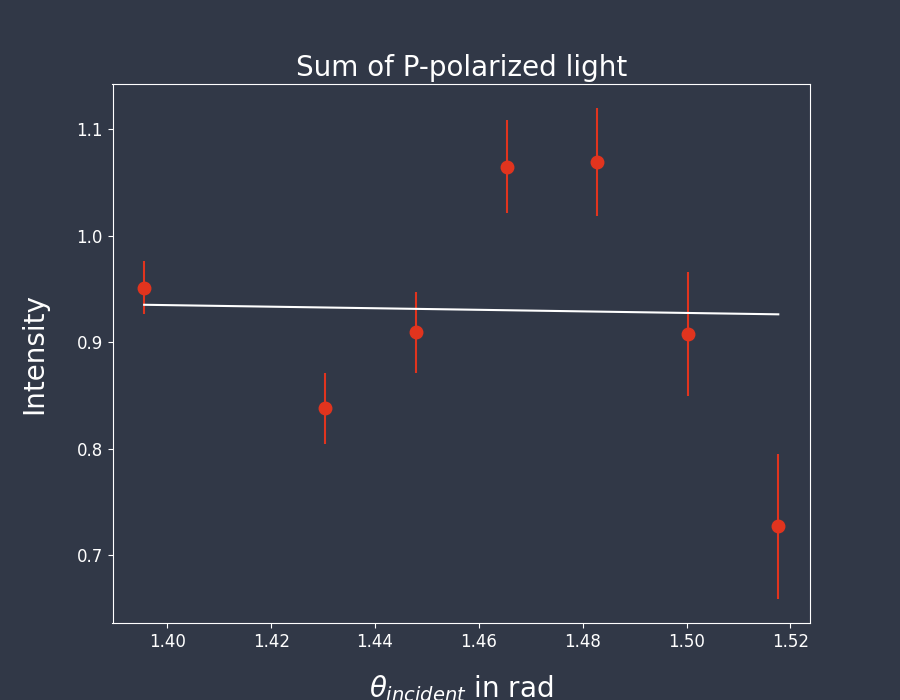
\includegraphics[width=\textwidth]{../PSum}
\end{figure}
\begin{figure}[H]
	\centering
	\sidecaption{The data for s-polarized light. This data does not seem to be constant either.}
	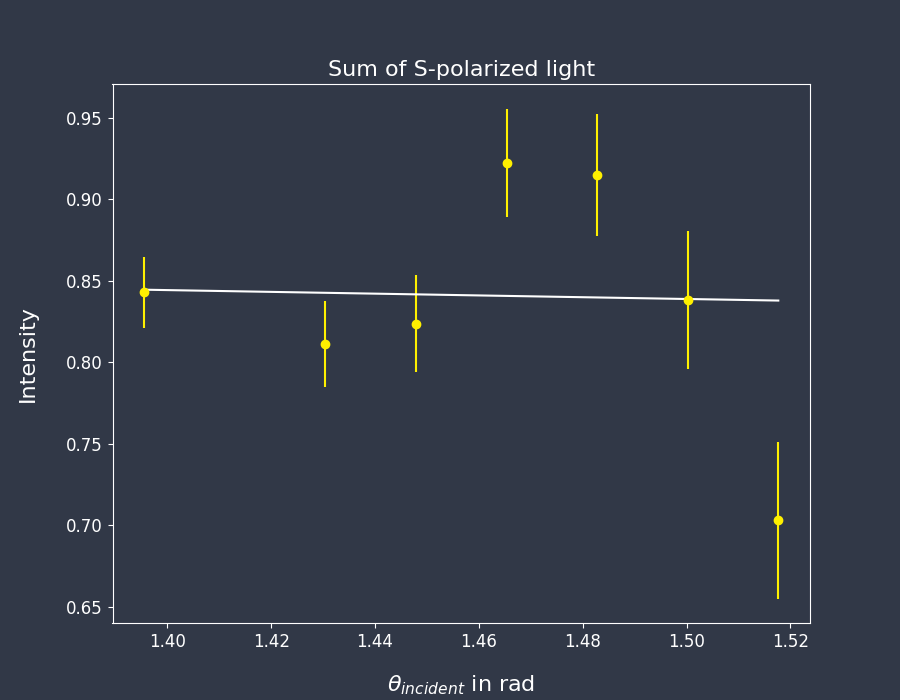
\includegraphics[width=\textwidth]{../SSum}
\end{figure}
For some reason, our data was unable to prove this. The intensities of the transmitted and reflected light seem to be somewhat out of sync. Due to background noise, only very few datapoints can be mutually accurate for both the transmitted and reflected intensities (an accurate datapoint necessitates a high intensity). We have chosen not to plot the error of the fit, as the magnitude of this error obscures the plot 
\newpage

\subsection*{Discussion}
As we have said before, the most influential inherent uncertainty in this experiments, comes from measuring the angles of incidence and transmission. The uncertainty is in itself not particularly disturbing. For a demonstration of Snell's law, the protactor is sufficiently precise. However, when demonstrating more complex relations, the uncertainty is propagated and therefore starts to obscure the connections. In particular, the measurements of conservations of intensity would benefit from a protractor with higher resolution. \\
Our data collected for the reflected was in general quite good, although we would have benefitted from collecting data for a larger variety of angles. Our data from the transmitted light seems to be afflicted by a systematic error, as all our datapoints lie a bit below the curve. This might be due to the glass absorbing a fraction of the light passing through it. 
Another problem, was our inability to give a conclusive estimate for the error in the intensity. This is crippling, as the statistical methods we have been taught, rely upon an accurate assessment of the errors in the dependent variables (curve-fit and chi-squared). The error we could measure was, was in the indepencent variable (the angle). Our solution to this problem, was to propagate the error measured in the independent varable, and use this as an estimate for the error in intensity. This is however, \textit{only} a good estimate when the propagating function describes a \textit{true} relation. So this method should not be considered good general practice. In the future, we should familiarize ourselves with a larger variety of statistical methods and not always resort to propagation. \\
Our data comparing the sums of intensities, is not very accurate. Interestingly, the two datasets describing P-polarized and S-polarized light seem to be correlated. This implies that the same error afflicts and in turn that the error is systematic. Our best guess, is that the background noise interferes with our measurements for the transmitted light at high angles. This makes sense, since the transmitted light has relatively low frequency at these angles. Furthermore, the background noise obscures S- and P polarized light equally.
We had some general issues while doing this experiment that ended up influencing the amount of data we were able to collect and how familiar we became with the general setup of the experiment. The first week of the exercise we both had Corona and the second week we had issues with different components of the experiment malfunctioning. Given more time, we would certainly have been able to take more and better data.
\subsection*{Conclusion}
Let us consider the different parts of the experiment. Our data seems to follow Snell's law, with predictable reasonable deviations. Our data also seems to follow the Fresnel relations reasonably well. However, the lack of points at low intensities, as well as the larger uncertainties, do mean that we are less confident that the relation holds. Our lack of points measuring the sum of intensities, as well the huge errors stemming from combining the datasets, mean that we can not conclude with any confidence with any confidence that this is conserved. Nor that it is not conserved. In order to say anything meaningful, we would have to collect more data.
\printbibliography
\end{document}
